\section{The response generated by aggregation}
\label{hrec:sec:aggregation}
Let \(u\) be a broadcast signal and let the \(N\) detector outputs be \(\sigma_i\in\{-1,1\}\). Conditional on a fixed \(u\), assume they are independent with
\begin{equation}
 p(u)=\Pr(\sigma_i=1\mid u)=\frac{1+\tanh(\beta u)}2,\qquad \beta>0.
 \label{hrec:eq:detector}
\end{equation}
Here \(\beta\) has inverse-signal units. We define the collective response as the \emph{mean verdict}, the expected sign of the population vote:
\begin{equation}
 R_N^{\rm ex}(u)=\E\!\left[\operatorname{sign}\Bigl(\sum_{i=1}^N\sigma_i\Bigr)\,\middle|\,u\right].
 \label{hrec:eq:majority}
\end{equation}
For even \(N\), ties have expected verdict zero. A literal zero verdict and a fair binary tie-break have the same mean, but not the same variance or the same closure under further aggregation. We use odd blocks when constructing a nested binary hierarchy.

The slope at zero measures how strongly a small broadcast changes the expected vote. Differentiating a configuration probability at zero multiplies it by \(\beta\sum_i\sigma_i\). Consequently
\begin{align}
 G_N^{\rm ex}
 &=\bigl(R_N^{\rm ex}\bigr)'(0)=\beta\,\E|S_N|,\qquad S_N=\sum_i\sigma_i,\nonumber\\
 &=\beta N\,\frac{\binom{N-1}{\lfloor(N-1)/2\rfloor}}{2^{N-1}}.
 \label{hrec:eq:exact-slope}
\end{align}
Appendix~\ref{hrec:app:majority} derives the last equality. Its leading behaviour is \(\beta\sqrt{2N/\pi}\). The relative correction is \(+1/(4N)\) for odd \(N\) and \(-1/(4N)\) for even \(N\). Thus even the first correction remembers the actual finite voting rule.

For comparison, the arithmetic mean \(N^{-1}\sum_i\sigma_i\) has expectation \(\tanh(\beta u)\), whose origin slope is simply \(\beta\). Averaging and thresholding do different things. The average has variance \(1/N\) at zero bias, while an odd-population binary majority verdict has variance one. A steep \emph{mean} verdict is not a nearly noiseless single verdict. Throughout the dynamical calculations below, a response such as \(R_N\) is used deterministically as an expected control action. A physical implementation would need enough repeated samples, or an explicit stochastic model, to justify that replacement.

Two smooth responses will let us exhibit the controller distinction analytically:
\begin{equation}
 \begin{aligned}
 f_N(\theta)&=\erf\!\left(\sqrt{N/2}\sinh(\beta\theta)\right),\\
 R_N(u)&=\erf\!\left(\beta\sqrt{N/2}\,u\right).
 \end{aligned}
 \label{hrec:eq:proxies}
\end{equation}
The error function is \(\erf(v)=2\pi^{-1/2}\int_0^v e^{-t^2}\,dt\). Both origin slopes equal \(\beta\sqrt{2N/\pi}\), but the functions are not identical. We treat each as an exactly specified deterministic model, not as an exact finite-binomial response. A Gaussian approximation to physical majority blocks would additionally require control of the approximation at every block and of its derivative through the composition. The exact tree calculation in Sec.~\ref{hrec:sec:hierarchy} needs no such approximation.

\section{Closing the adaptive loop}
\label{hrec:sec:loop}
The first placement makes the population response part of a relaxing report. At integer update \(k\), let \(m_k\) be that report and \(\theta_k\) the broadcast. Let \(M(\theta)\) denote its stationary plant response and \(F(\theta)\) the response the controller expects. The lagged gradient-mismatch map is
\begin{align}
 m_{k+1}&=r m_k+(1-r)M(\theta_k),\nonumber\\
 e_k&=m_k-F(\theta_k),\nonumber\\
 \theta_{k+1}&=\theta_k+\alpha F'(\theta_k)e_k.
 \label{hrec:eq:lagged}
\end{align}
The parameter \(0\le r<1\) is the retained fraction of the old report. For an exponentially relaxing plant observed every \(T>0\) with relaxation time \(\tau>0\), \(r=e^{-T/\tau}\). We do not require the additional limit \(T\gg\tau\). The positive step \(\alpha\) has units \([\theta]^2/[m]^2\). With \(m\) held fixed, the last line is a gradient step on \(\tfrac12[m-F(\theta)]^2\), not gradient descent on an asserted global objective for the coupled system. Crucially, it uses \(m_k\), not \(m_{k+1}\).

Suppose \(M(\theta_*)=F(\theta_*)=m_*\), and write \(s=M'(\theta_*)\), \(b=F'(\theta_*)\). For \(C^2\) responses the equilibrium Jacobian in state order \((m,\theta)\) is
\begin{equation}
 J_{\rm lag}=
 \begin{pmatrix}r&(1-r)s\\ \alpha b&1-\alpha b^2\end{pmatrix}.
 \label{hrec:eq:lagged-jacobian}
\end{equation}
The linear mismatch obeys
\begin{equation}
 \delta e_{k+1}=(r-\alpha b^2)\delta e_k+(1-r)(s-b)\delta\theta_k.
 \label{hrec:eq:linear-mismatch}
\end{equation}
Point equality supplies an equilibrium. Equal slopes \(s=b\) additionally supply linear eigenvalues \(1\) and \(r-\alpha b^2\). They do not supply a family of equilibria. For example, \(M(\theta)=\theta+\theta^3\), \(F(\theta)=\theta\) match in value and slope at zero, yet their only intersection is zero. A fixed curve requires the stronger \emph{functional} identity \(M=F=f\) on a neighbourhood. In that case every \((f(\theta),\theta)\) is fixed, and the eigenvalue one represents motion tangent to that curve.

The second placement uses the detector population to convert a newly observed plant mismatch into a control action. Let \(x_k\) be a scalar plant state, let its stationary response be \(s\theta\), and let \(b\theta\) be the target, with \(b>s>0\). Using a positive response step \(\varepsilon\), define
\begin{align}
 x_{k+1}&=r x_k+(1-r)s\theta_k,\nonumber\\
 u_k&=x_{k+1}-b\theta_k,\nonumber\\
 \theta_{k+1}&=\theta_k+\varepsilon R_N(u_k).
 \label{hrec:eq:post}
\end{align}
Here \(R_N\) is dimensionless, \([\varepsilon]=[\theta]\), and \(s,b\) both have units \([x]/[\theta]\). Thus \(K=\varepsilon R_N'(0)\) has units \([\theta]/[x]\), and \(Kb\) is dimensionless. The sign convention makes a negative mismatch lower \(\theta\). For a strictly increasing odd \(R_N\), the only equilibrium is \((0,0)\): stationarity requires \(x=s\theta=b\theta\).

\begin{figure*}[t]
 \centering
 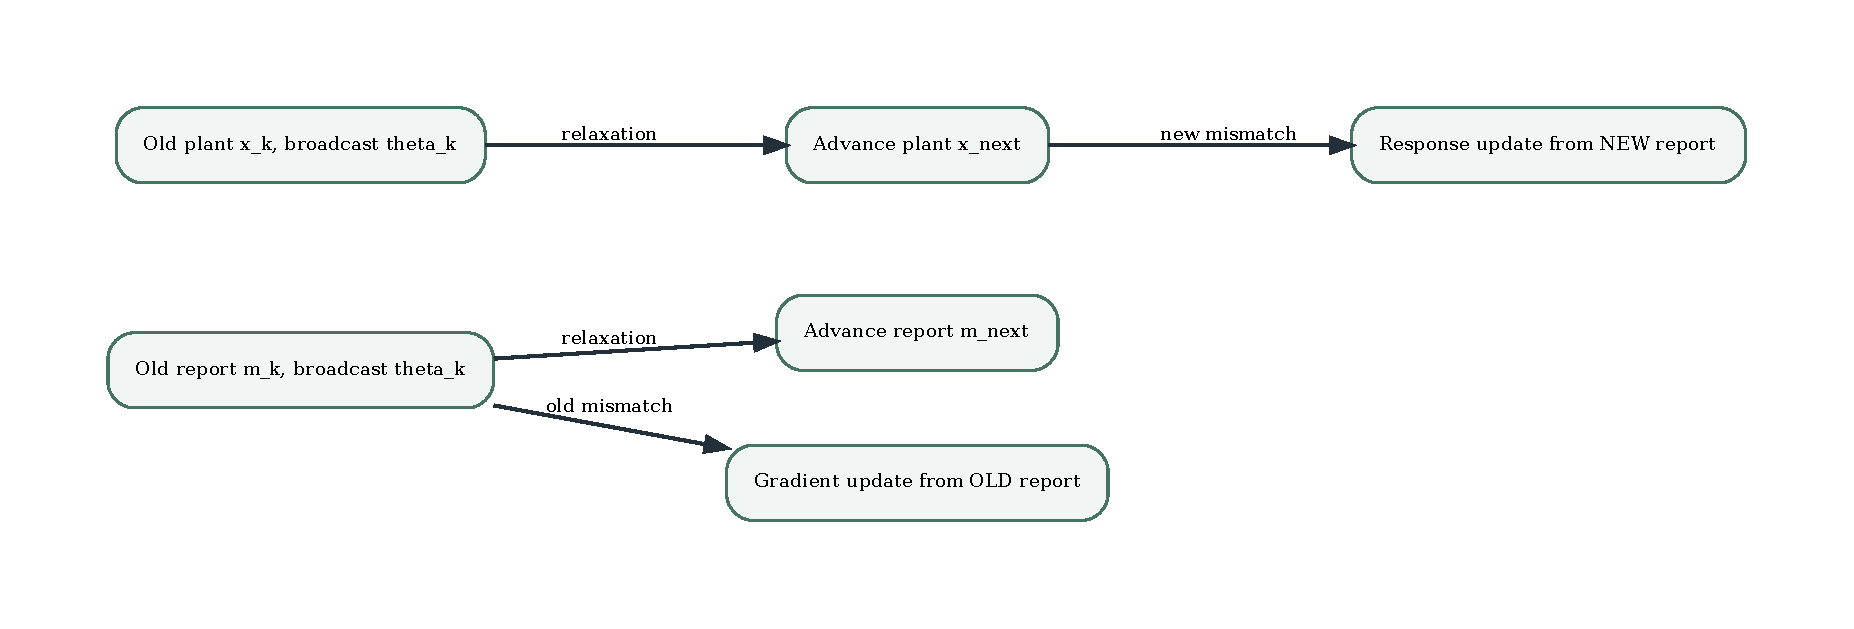
\includegraphics[width=\textwidth]{figures/generated/hierarchy-controller-timing-paper.pdf}
 \caption{The response must be located in time before its gain is calculated. In the lagged map, the plant advance and control update consume the old pair \((m_k,\theta_k)\). In the post-observation map, the plant advances first and its new state enters the response-driven update. The maps are Eqs.~\eqref{hrec:eq:lagged} and \eqref{hrec:eq:post}, respectively. Neither path is an elimination of the other.}
 \label{hrec:fig:timing}
\end{figure*}

Writing \(c_p=(1-r)s\), \(\Delta=b-c_p\) and \(K=\varepsilon R_N'(0)\), the second equilibrium Jacobian is
\begin{equation}
 J_{\rm post}(K)=
 \begin{pmatrix}r&c_p\\Kr&1-K\Delta\end{pmatrix}.
 \label{hrec:eq:post-jacobian}
\end{equation}
Only one response derivative enters \(K\). By contrast, functional matching in Eq.~\eqref{hrec:eq:lagged} gives the dimensionless transverse gain \(K_{\rm lag}=\alpha f'(\theta)^2\). The second derivative factor is not an extra population mechanism. It comes from choosing the target-gradient controller as well as a response-dependent plant. Figure~\ref{hrec:fig:timing} keeps this distinction visible.

